\documentclass[usegeometry=true]{scrartcl}
 \usepackage{csquotes}
\usepackage[ngerman]{babel}
\usepackage[T1]{fontenc}
\usepackage{lmodern}
\usepackage[utf8]{inputenc}
\usepackage{hyperref}
\usepackage{amssymb}

% Dimensionen bitte nicht ändern. 
\usepackage[left=2cm, right=2cm, top=2cm, bottom=2cm, bindingoffset=1cm, includeheadfoot]{geometry}
%Zeilenabstand bitte nicht ändern
\usepackage[onehalfspacing]{setspace}
\usepackage{graphicx}
\usepackage[backend=biber,style=numeric,]{biblatex}\addbibresource{literatur.bib}

\begin{document}
% ----------------------------------------------------------------------------
\subject{Projektbericht zum Modul Information Retrieval und Visualisierung Sommersemester 2023}
\title{Visualisierungen zur Analyse von Einflussfaktoren auf die Schlaff Effizienz}
%\subtitle{Untertitel}% optional
\author{Mick Stewart Wörner}% obligatorisch
\date{28.12.2023}\dedication{\normalsize\vfill\hrule\vspace{20pt}
    Link zum GitHub-Repository (URL des Projekt):\\
    \url{https://github.com/EinKnopfzu/Sleep-Efficiency-Dataset/tree/main}\\
    Letzter Commit: \\
    Datum Commit: 28.12.2023 - 22:37\\
}
\maketitle% verwendet die zuvor gemachte Angaben zur Gestaltung eines Titels
% ----------------------------------------------------------------------------
% Inhaltsverzeichnis:
%\tableofcontents
% ----------------------------------------------------------------------------
% Gliederung und Text:
\newpage
\section{Einleitung}
 Im folgenden Paper werden drei Visualisierungstechniken zur Analyse von Schlafqualität dargestellt. Dabei wird ein Fokus auf die Analyse der Verteilung, Einflüsse und Korrelation mit Verhaltensweisen gelegt. Die vorgestellten Visualieirungen ermöglichen es dem Anwender ein tiefes Verständinis über die Aussagefähigkeit der Daten und Zusammenänge zu erschaffen.
\subsection{Anwendungshintergrund}
Hintergund dieser Anwendung ist die Darstellung von im Internet bereitgestellten Daten. Diese beziehen stellen unterschiedliche Attribute zur Beschreibung der Schlafqualität dar un derhebt  dazu Daten zu verschiednenen verhaltensweisen. Die Daten können durch die Visualisierung beurteilt, in Kontext gesetzt und mit verhaltensweisne korreliert werden.  
\subsection{Zielgruppen}


Die Schlafqualität spielt eine entscheidende Rolle für die Lebensqualität, deswegen richtet sich die Anwendung 
an eine Zielgruppe, die ein Interesse daran hat, die Zusammenhänge und Einflüsse auf die Schlafqualität zu verstehen.
 Diese Zielgruppe könnte aus Forschern und Privatpersonen bestehen, die daran interessiert sind, wie verschiedene 
 Lebensstile die Schlafqualität beeinflussen können und die Schlafzyklen sich zueinander Verhalten.
 Ein tiefgehendes Wissen über die Schlafphasen ist nicht erforderlich, aber ein generelles Interesse an der Analyse des Zusammenhangs zwischen Verhalten und Schlafqualität charakterisiert den Benutzer.
 Die Benutzer sollten sich darüber im Klaren sein, dass die Visualisierungen Hinweise liefern können, 
 jedoch nicht notwendigerweise kausale Zusammenhänge zeigen.

Die Visualisierungen, die in diesem Projekt präsentiert werden, sollen dabei helfen, Einflüsse und Zusammenhänge
 bei der Schlafqualität zu identifizieren. Dabei werden verschiedene Attribute wie Koffein-, Alkohol- und Tabakkonsum
 , Sport, sowie Alter und Geschlecht der Personen untersucht. Die Zielgruppe sollte ein Grundverständnis
  für die Bedeutung dieser Attribute in Bezug auf die Schlafqualität haben.

Die Benutzer sollten sich bewusst sein, dass der Datensatz, der in dieser Anwendung verwendet wird,
 nur 452 Personen umfasst und durch die Datenverarbeitung weiter reduziert wird. 
 Daher ist es wichtig, die statistische Validität der Ergebnisse zu berücksichtigen,
  insbesondere bei der Anwendung von Filtern. Statistische Aussagekraft ist bei n <30 nicht mehr gegeben,
   und daher müssen die Benutzer dies bei der Benutzung berücksichtigen.



\subsection{Überblick und Beiträge}
Im diesem Abschnitt wird eine Überblick auf die Daten und verwendeten Visualisierungstechniken gegeben. 

\section{Daten}

Der verwendete Datensatz bietet eine umfangreiche Sammlung von 15 Attributen, die Informationen 
über die Schlafqualität und Lebensgewohnheiten von 452 Personen liefern.
Auf der Kaggle Seite wird nach Angaben des Authors behauptet, dass der Datensatz im Kontext einer Studie von der ENSIAS, Marroco gesammelt wurde.
Innerhalb einer Literatur Recherche konnten weder auf der Webseite der ENSIAS noch in weitergehender Literaturrecherche eine Veröffentlichung zu diesem Datensatz identifizieren.
Daher sollten die Daten und daraus entwickelten Ergebnisse, nicht unreflektiert übernommen werden. 

Der Datensatz hat drei Nominale (Id, Gender und Raucher) und zwölf Quantitative (Age, Bedtime, Wakeup Time, Sleep Duration, Sleep Efficiency, REM Sleep percentage, Deep Sleep Percentage, Light Sleep Percentage, Awakenings, Caffeine Intake,Alkohol Intake, Tobako Intake, Exercise frequency) Aufgrund der unklaren Herrkunft des Datensatzes muss werden die Attribute im folgenden näher beschrieben.\\
\begin{itemize}
  \item ID: Die ID identifiziert eine Person eindeutig. Da keine ID mehrfach aufgeführt wurde, ist anzunehmen, dass jede Person nur einmal an der Studie teilgenommen hat. Die ID wird als Integer bereitgestellt, und der Datenbereich reicht von 1 bis 452.
  \item Age: Gibt das Alter an, das die Person zum Zeitpunkt der Erfassung hatte. Das Alter wird als Integer angegeben und ist daher diskret, zum Beispiel 43 Jahre. Die Verteilung des Datenbereichs wird im Folgenden in diesem Format angegeben: (Quantile [Min, 25, 50, 75, Max]), Quantile [9, 29, 40, 52, 69].
  \item Gender: Das Geschlecht wird als String abgespeichert und nimmt nur zwei Werte an: ''Male'' oder ''Female''. Dabei gibt es einen Anteil von 50 Prozent Männern und 50 Prozent Frauen.
  \item Bedtime: Gibt die Uhrzeit an, zu der die Person ins Bett gegangen ist. Hierbei ist nicht klar, ob damit der Zeitpunkt gemeint ist, zu dem die Person eingeschlafen ist oder zu dem die Person sich ins Bett gelegt hat. Die Information werden als DateTime angegeben. Die Daten steigen in 30 Minuten schritten und ist trotz DateTime Formati damit Diskret. 
  \item WakeUp time: Gibt das Datum und die Uhrzeit an, zu dem die Person erwacht. Steigt analog zu der Bedtime in halben Stunden Schritten an. Das Datum ist bei beiden DateTime-Formaten nicht von weiterem Interesse, da es keine zeitliche Entwicklung der erfassten Personen gibt.
  \item Sleep Duration: Die Schlafdauer ist wie die Bedtime unklar in ihrer Interpretation, da sich der Wert immer aus der Differenz zwischen Bedtime und WakeupTime berechnet. Daher ist unklar, ob es sich um die geschlafene oder um die im Bett verbrachte Zeit handelt. Die Spalte wird als Float angegeben und steigt aufgrund der halbstündlichen Sprünge der BedTime und WakeupTime auch in 0.5 Schritten. Die Daten haben Quantile von [5.0, 7.0, 7.5, 8.0, 10.0] Stunden. Die Interpretation der Sleep Duration wird weiter dadurch erschwert, dass im weiteren Datensatz die Anzahl angegeben wird, wie oft eine Person in der Nacht wach wird, ohne Angabe, wie lange diese "Schlafpausen" spezifisch sind.
  \item Sleep efficiency: Gibt den prozentualen Anteil an, den eine Person schlafend im Bett verbracht hat. Die Daten werden als Float mit zwei Nachkommastellen angegeben. Die Daten haben die Quantile: [0.5, 0.7, 0.82, 0.9, 0.99]. Eine Person, die 5 Stunden im Bett verbracht hat und davon eine Stunde wach war, hat also eine Schlafeffizienz von 80 Prozent. Da hier wieder eine Interpretationsproblematik besteht, wird im weiteren davon ausgegangen, dass die Schlafeffizienz angibt, welchen Anteil die Person nach erstmaligem Einschlafen, schlafend verbringt. Weiter wird diese Kennzahl in der Datenverarbeitung auf einen absoluten Stundenwert hochgerechnet.
  \item REM Sleep percentage: Die REM steht für Rapid Eye Movement Schlaf, dies ist einer der drei Schlafzyklen, die ein Mensch im Schlaf durchführt. Die CDC empfiehlt einen Anteil von 25 Prozent \href{https://www.healthline.com/health/how-much-deep-sleep-do-you-need}{Healthline} . Der REM Percentage gibt den prozentualen Anteil an, den die schlafende Person im REM verbracht hat, also den Anteil REM an Schlaf Effizienz. Die Daten werden als Integer abgespeichert und haben Quantile von [15, 20, 22, 25, 30]. Weiter wird diese Kennzahl in der Datenverarbeitung auf einen absoluten Stundenwert hochgerechnet.
  \item Deep sleep percentage: Der Tiefschlaf-Prozentsatz gibt den Anteil am Schlaf an, der im Tiefschlaf verbracht wurde. Die Daten werden als Integer angegeben und haben Quantile von [18, 51, 58, 63, 75]. Weiter wird diese Kennzahl in der Datenverarbeitung auf einen absoluten Stundenwert hochgerechnet.
 \item Light sleep percentage: Gibt den prozentualen Anteil am Schlaf an, der im Leichtschlaf verbracht wurde. Die Daten werden als Integer angegeben und haben Quantile von [7, 15, 18, 40, 63]. Weiter wird diese Kennzahl in der Datenverarbeitung auf einen absoluten Stundenwert hochgerechnet.
 \item Awakenings: Gibt die absolute Anzahl an, wie oft eine Person aufgewacht ist. Die Daten werden im Datensatz als Float abgespeichert. 0.0 bedeutet, dass eine Person durchgeschlafen und nur einmal final am Morgen aufgewacht ist. Die Daten reichen von [0.0, 1.0, 1.0, 3.0, 4.0].
 \item Caffeine intake: Gibt an, wie viel Koffein die Person in den letzten 24 Stunden zu sich genommen hat. Die Maßeinheit hierbei beträgt mg. Die Daten werden als Float abgespeichert und haben Quantile von [0.0, 0.0, 25.0, 50.0, 200.0].
 \item Alcohol intake: Gibt an, wie viel Alkohol die Personen in den letzten 24 Stunden zu sich genommen haben in Oz. Die Daten haben Quantile von [0.0, 0.0, 0.0, 2.0, 5.0].
 \item Tobacco intake: Gibt an, ob die Person raucht. Die Daten sind als String abgespeichert: "Yes" für Raucher und "No" für Nichtraucher. 154 Personen geben an zu rauchen und 298 geben an Nichtraucher zu sein.
 \item Exercise frequency: Gibt an, wie viele Einheiten Sport die Person in der Woche macht. Dabei ist nicht angegeben, welche Maßeinheit diese Einheiten Sport haben. Die Daten haben Quantile von [0, 0, 2, 3, 5], es gibt 6 fehlende Werte.
\end{itemize}

Unter der Annahme, dass die Daten valide sind und die angegebene Interpretation der Attribute korrekt ist, gewährt dieser Datensatz detaillierte Einblicke in die Schlafqualität, insbesondere hinsichtlich der Schlafphasen und ihrer Dauer. Allerdings weist die Erfassung der Kaffee- und Alkoholeinnahme Schwächen auf, da diese Substanzen im menschlichen Körper eine geringe Halbwertszeit haben, und somit der zeitliche Kontext der Einnahme relevant wäre. Weitere Einflussfaktoren auf die Schlafqualität werden nicht erfasst, ebenso wenig wird die Länge individueller Schlafunterbrechungen differenziert oder den drei Schlafphasen zugeordnet. Daher könnte es für den Anwender von Interesse sein zu erfahren, welche der Schlafphasen durch bestimmte Verhaltensweisen gestört werden. Zudem lässt sich argumentieren, dass die Verteilung der Verhaltensweisen sehr linksseitig ist, dies ist möglicherweise auf kulturelle Unterschiede zurückzuführen. Daher sollte die Aussagekraft des Datensatzes auf den marokkanischen Lebensstil eingeschränkt werden.
\section{Die Daten}
  Der Datensatz wurde auf \href{https://www.kaggle.com/datasets/equilibriumm/sleep-efficiency/data}{Kaggle} veröffentlicht und ist die dritte Version. Die Daten sind als CSV mit einer Größe von 9 kB zugänglich. Sie sind im GitHub-Repository abgelegt, was eine zentrale Aktualisierung der Daten ermöglicht, falls dies notwendig sein sollte.

 Das Programm ruft die CSV-Datei mittels eines HTTP-GET-Requests auf und speichert sie als einen String ab. Falls der Request erfolgreich ist, wird die Nachricht `Got Text Ok fulltext' an die Funktion `update` gesendet. Der String wird dabei durch `fullText' repräsentiert. Daraufhin wird im `Model' das `datenladen' auf `Success' gesetzt.
 Auf den String wird die Funktion `stringtoUnverarbeitete' angewandt, deren Ziel es ist, den String in eine `Liste (UnverarbeiteteDaten)' zu transformieren. Die Funktion verwendet das Paket `BrianHicks/elm-csv' (im Code als Decode bezeichnet), um die Namen der Felder aus der ersten Zeile im String zu extrahieren. Die Funktion `decode' decodiert die Eingabedaten, wobei zu beachten ist, dass auch leere Felder im String vorkommen dürfen. Die Funktion `Decode.blank' gibt ein `Nothing' zurück, falls das Feld leer ist. Wenn es dennoch zu einem Fehler kommt, gibt die Funktion `stringtoUnverarbeitete' eine leere Liste an das Modell zurück.
 Wenn die Daten nun in Form von `UnverarbeiteteDaten' vorliegen, wird die Funktion `sleep2Point` angewandt. Diese entfernt ein Tupel, wenn eines seiner Felder ein `Nothing' enthält. Weiter werden die Werte für REM, Tiefschlaf und Leichtschlaf in tatsächlich verbrachte Stunden transformiert, indem sie mit 0.1 in Prozent umgerechnet und dann mit der Schlafeffizienz und Schlafdauer multipliziert werden. Dies verbessert die Interpretierbarkeit und stellt die Vergleichbarkeit her.
 Gender und Raucher werden von einem String zu einem Float mittels Case-Handling konvertiert (Funktionen `genderToFloat' und `raucherToFloat'). Dies ermöglicht das Rechnen mit den Daten und erleichtert die weitere Visualisierung.
 Die Funktion `sleep2Point' hat einen Output vom Typ Alias `AussortierteDaten`. Weiter werden die Attribute Bedtime und Wakeup Time in den aktuellen Visualisierungen nicht verwendet, könnten jedoch bei der Weiterentwicklung interessant werden. Daher wurden sie im Datenkonstrukt belassen, aber nicht weiter behandelt – man könnte von einer sanften Projektion sprechen. Innerhalb der Einstellungen kann der Anwender eine Selektion durchführen und Einschränkungen auf das zu untersuchende Attribut anwenden. So werden nur Datentupel an die Visualisierungen übergeben, die dem Kriterium entsprechen.


   
\newpage
\section{Visualisierungen}
\subsection{Analyse der Anwendungsaufgaben}

Die konkreten Anwendungsaufgaben, die von den Anwendern bearbeitet werden müssen, zielen darauf ab, die Daten kritisch zu analysieren, Zusammenhänge zwischen verschiedenen Attributen explorativ zu erkennen und den Einfluss der Verhaltensweisen zu erkennen.
\begin{enumerate}
  \item Datenlage analysieren:
  \begin{itemize}
    \item    Die Nutzer müssen zunächst die Datenlage kritisch analysieren und die Güte der einzelnen Attribute bewerten. Hierbei ist ein Verständnis für die statistische Interpretation und die Relevanz von Normalverteilungen zur Aussagefähigkeit der Visualisierungen wichtig.

  \end{itemize}
  \item Vergleich von Attributen:
  \begin{itemize}
    \item Nach der Bewertung der Güte der Attribute, soll ein Nutzer den Zusammenhang dieser mit anderen Attributen verstehen. Es soll hierbei auch auf versteckte Zusammenhänge stoßen können und die indirekte Beziehungen erkennen. 
  \end{itemize}
  \item Analyse der Einflüsse des Verhaltens:
  \begin{itemize}
    \item Die Einflüsse des Verhaltens auf die Attribute müssen analysiert werden. Hierbei ist es notwendig, den Einfluss von multiplen Verhaltensindikatoren auf die Ausprägung eines Merkmals zu schätzen.
  \end{itemize}
\end{enumerate}
Bei diesen Aufgabe sind die folgenden mentalen Modelle von Bedeutung:

\begin{enumerate}
  \item Statistische Interpretation:
  \begin{itemize}
    \item Nutzer sollten Grundlagen der statistischen Interpretation und die Relevanz von Normalverteilungen verstehen. Visualisierungen wie QQ-Plots können dabei helfen, Abweichungen von der Normalverteilung zu identifizieren.
  \end{itemize}
  \item Korrelation interpretieren:
  \begin{itemize}
    \item Ein Verständnis für die Interpretation von Korrelationen ist wichtig. Visualisierungen können durch Farbgebung (z. B. Rot für negative und Grün für positive Korrelationen) unterstützen, auch wenn dies nicht zwingend notwendig ist.
  \end{itemize}
  \item Parallele Koordinaten Interpretieren:
  \begin{itemize}
    \item Benutzer sollten verstehen, dass jede Achse ein Attribut repräsentiert, und Linien zwischen den Achsen die Beziehung zwischen Werten in verschiedenen Dimensionen anzeigen. Die Interpretation von Parallelenkoordinaten erfordert die Fähigkeit, Muster in den Linienverläufen zu erkennen und so Zusammenhänge zwischen den Attributen zu verstehen.
  \end{itemize}
\end{enumerate}


\subsection{Anforderungen an die Visualisierungen}
Die Visualisierungen müssen die Anwenderinnen bei der explorativen Analyse unterstützen. Somit müssen die Daten expressiv und effektiv dargestellt werden. 
Die Visualiserung muss die Daten korrekt wieder geben,, dabei den Anwender  unterstützen, Muster und Trends in den Daten zu identifizieren.
Weiter müssen die Attribute sinnahfting auf Ihre Beziehungen unteinander Darsgestellt werden und die Anwenderin dabei unterstützen auch indirekte Beziehungen zu erkennen. 
Ausßerdem müssen die Visualisierungen die Einflüsse der Verhaltensweisen auf die Schlafqualität leicht interpretierbar darstellen.
Die Visualisierungen sollten barrierefrei gestaltet sein, um sicherzustellen, dass Benutzer mit unterschiedlichen visuellen Fähigkeiten die Informationen analysieren können.


\textbf{ Anforderungen an das Design. }
\subsection{Präsentation der Visualisierungen}

Im folgenden Abschnitt weren die drei verwendeten Visualiseungs Techniken vorgestellt, deren Nutzen für den Anwender dargelegt und alternative Visualisierungen besprochen.

\subsubsection{Visualisierung Eins: QQ-Plot Datenlage Normalverteilt?}

Die erste Visualisierung ist die Darstellung der Daten in einem zweidimensionalen Diagramm, spezifisch eines Normalverteilungs-QQ-Plots.

Ein QQ-Plot (Quantile-Quantile-Plot) ist ein nützliches grafisches Werkzeug in der statistischen Datenanalyse, insbesondere wenn es darum geht, die Verteilung von Daten zu überprüfen und diese mit einer theoretischen Verteilung zu vergleichen. In der Anwendung wird aufgrund des Implementierungsaufwandes nur der Vergleich mit der Normalverteilung vorgenommen. Hierzu werden die Daten berechnet, die Verteilung der Daten berechnet, die das Attribut hätte, falls es einer Normalverteilung folgen würde, und in einem Scatterplot dargestellt.

Die typischen Aufgabenfelder eines QQ-Plots sind die Normalitätsüberprüfung, die Identifikation von Abweichungen, die Bestätigung der Normalverteilungshypothese und Identifikation von Ausreißern.

Die Visualisierung zeigt den Wert auf der Y-Achse an, den ein Datenpunkt hätte, falls der Datensatz einer Normalverteilung folgen würde. Die X-Achse zeigt den Wert des Datenpunktes an. Dann werden die Datenpunkte basierend auf ihrer Reihenfolge im Scatterplot gezeichnet. Ein perfekt normalverteiltes Attribut würde somit eine gerade Linie im 45-Grad-Winkel ergeben.

Dies ermöglicht dem Anwender eine Normalitätsüberprüfung durchzuführen. Somit kann dieser sich ein eigenes Bild darüber machen, ob das Attribut normalverteilt ist und seinen Anforderungen entspricht. Bei einem perfekt normalverteilten Attribut würden im QQ-Plot alle Punkte auf einer `f(x) = x'-Linie liegen. Abweichungen von dieser Linie deuten auf Abweichungen von der Normalverteilung hin; Krümmungen und Biegungen weisen auf Verschiebungen hin. Hier ist es an dem Anwender, diese zu interpretieren. Die hypothetische `f(x) = x' - Linie ist zur Orientierung auch eingezeichnet. Weiter ist eine rote Linie vom 25. Quantil bis zum 75. Quantil eingezeichnet. Dies erleichtert dem Benutzer den Datensatz zu überprüfen und einer Verunsicherung durch die Abweichungen an den Extrema entgegenzuwirken.

Die Identifikation von Ausreißern kann im Normal QQ-Plot an den visuellen Enden identifiziert werden. Starke Abweichungen sind durch eine große Distanz zur schwarzen Linie erkennbar. Diese können durch das Filtern des Datenbereichs entfernt werden. Weiter ist es möglich, einen Vergleich verschiedener Verteilungen anzustellen. Dies ist aufgrund des Umfangs des Projektes nicht in der Anwendung implementiert, könnte dem Anwender aber einen Mehrwert bieten. Somit sollte der Anwender durch den Scatterplot in der Lage sein, die Datenverteilung und Interpretierbarkeit einzuschätzen und diese in geringem Maße mit den Filtern zu selektieren.

\begin{figure}[h]
  \centering
  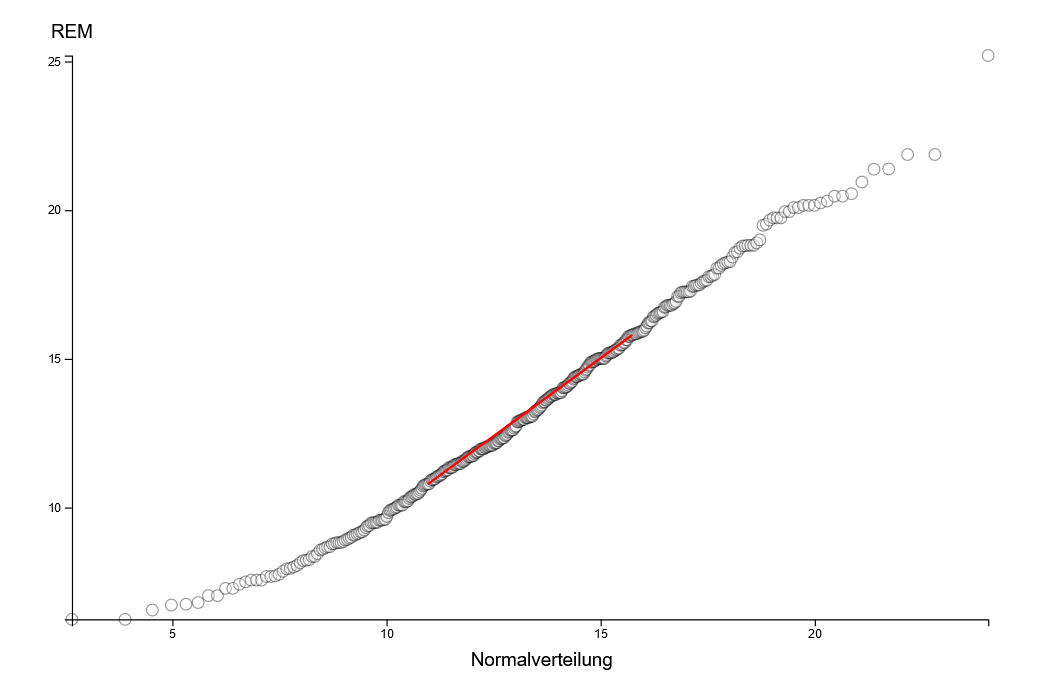
\includegraphics [width = 0.8\textwidth]{NormQQPlott.JPG}
  \caption{Visualisierung Eins  Norm QQ-Plot REM }
\end{figure}


Aufgrund des Anspruchs, die Interaktion von Daten analysieren zu können, sind zwei weitere Scatterplots unter dem des Hauptattributes dargestellt. Deren Funktion ist ebenfalls die Interpretation der Güte.

Das oben erwähnte Auswählen und das Filtern geschieht in der Seitenleiste. Hier kann der Benutzer das Attribut auswählen, das er untersuchen möchte, und direkt darunter dieses in seinem Wertebereich filtern. Die Seitenleiste wird im Abschnitt `Interaktion' genauer erklärt.
Der eingeschränkte Datenbereich wird dann in den anderen Visualisierungen verwendet.
Der Benutzer kann in der zweiten Visualisierung zwei weitere Attribute zum Untersuchen auswählen. Diese werden daraufhin unter dem Haupt-Scatterplot als kleinere QQ-Plots dargestellt. Dies ermöglicht auch für sie eine schnelle Einschätzung der Güte.

Die Visualisierung mittels Scatterplot ist im Kontext der Datenbewertung effektiv, da sie die zugrunde liegenden Fragestellungen visuell gut unterstützt und dem Anwender bei multiplen Fragestellungen Antworten liefern kann. Die Expressivität ist limitiert, da die Interpretation nicht ohne Kenntnis der Interpretation von QQ-Plots möglich ist und möglicherweise die Attribute, welche in den kleinen Scatterplots eine Unterordnung zum Haupt-Scatterplot impliziert.
Alternativ hätte auch ein Histogramm verwendet werden können. Bei diesem hätte man die Hürde zur Analyse reduziert, aber die Identifikation von Ausreißern erschwert.



\subsubsection{Visualisierung Zwei: Parallele Koordinaten}
Präsentieren der Visualisierung und Interaktionsmöglichkeiten. 

In der Visualisierung werden drei Dimensionen abgebildet: das im QQ-Plot ausgewählte Hauptattribut sowie zwei weitere Attribute. Die Achsen sind parallel zueinander angeordnet und gleich groß. Um die Ausprägungen eines Datentupels darzustellen, wird die Ausprägung des Tupels am jeweiligen Attribut auf die Y-Achse skaliert. Anschließend wird eine gerade Linie zwischen den Positionen auf den benachbarten Achsen gezogen, wobei die Endpunkte der Liniensegmente mit den Attributwerten korrespondieren.

Das Hauptattribut, das in Visualisierung 1 ausgewählt wurde, befindet sich in der Mitte, das Y-Attribut auf der linken und das Z-Attribut auf der rechten Seite. Es wurde bewusst darauf verzichtet, weitere Attributsdimensionen hinzuzufügen. Dies dient einerseits dazu, dass der Anwender seinen Fokus auf die Analyse des Hauptattributes legt, und andererseits könnten bei mehr als 3 Attributen suggerierte Zusammenhänge entstehen, die nicht zwangsläufig vorhanden sein müssen. Eine Clusterung zwischen Dimension 1 und 2 sowie zwischen 2 und 3 bedeutet nicht zwangsläufig eine Clusterung zwischen 1 und 3. Dies wäre der Effektivität abträglich, da so Zusammenhänge suggeriert werden könnten, die nicht beabsichtigt sind.

Parallele Koordinaten eignen sich besonders gut für mehrdimensionale, quantitative und endliche Daten. Diese sind in unserem Datensatz gegeben. Die Visualisierung ermöglicht es dem Anwender, Muster und Trends in den Daten zu identifizieren, die auf Beziehungen zwischen den Attributen hinweisen. Zum Beispiel können parallele Linien auf eine starke Korrelation zwischen den entsprechenden Variablen hinweisen. Die Visualisierung ermöglicht es dem Anwender, Rückschlüsse auf den Zusammenhang von Attributen zu ziehen und diese mit Visualisierung 1 zu vergleichen. Die Untersuchung der Attribute und das Visualisieren kann mittels eines interaktiven Anpassens der Pixelgröße und RGBA-Werte erfolgen, dies ist nützlich, da viele der Inputdaten wenige unterschiedliche Wertausprägungen haben, was die Clusterung der Inputdaten erschwert. Um dennoch interessante Muster erkennen kann. So kann der Benutzer basierend auf seinen eigenen visuellen Bedürfnissen Anpassungen vornehmen. In Bild 3 wird dies vorgestellt.



\begin{figure}[h]
  \centering
  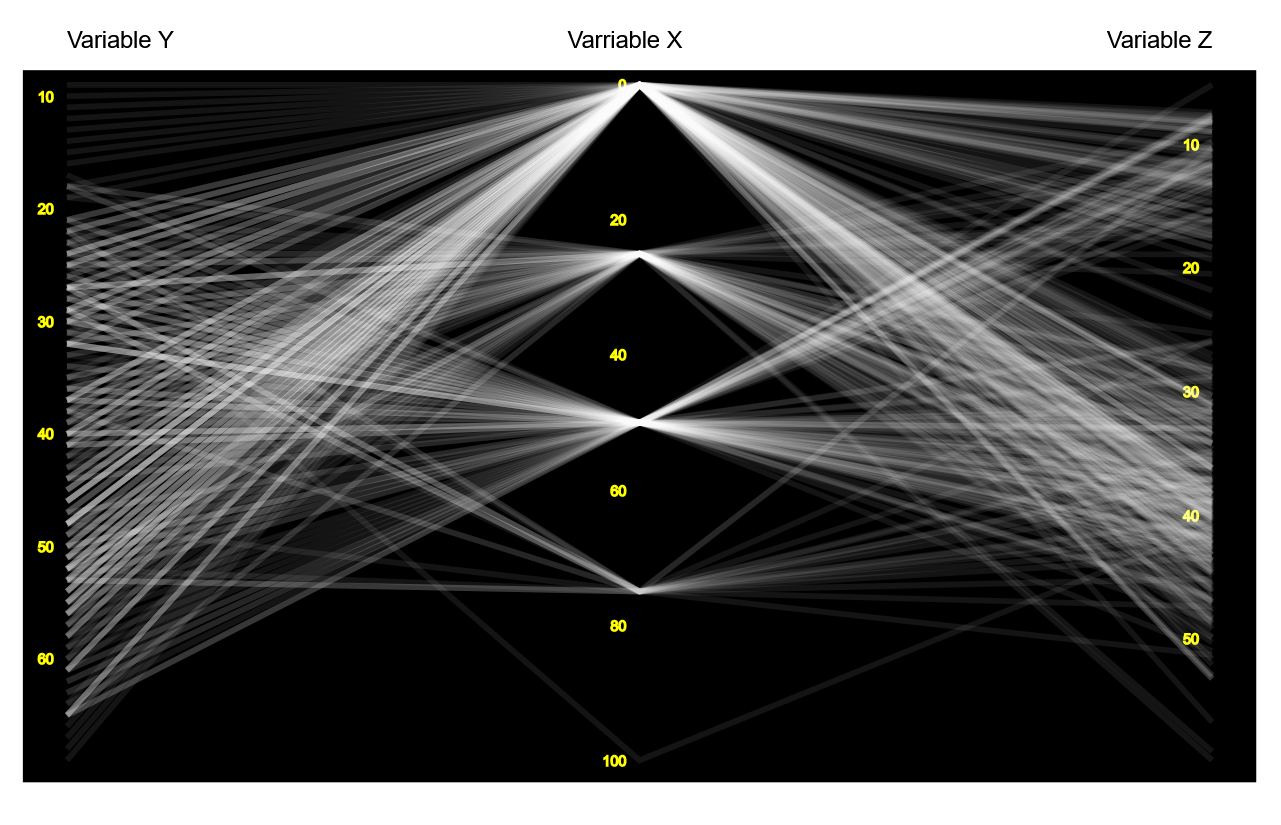
\includegraphics [width = 0.8\textwidth]{RoengtenBSP.JPG}
  \caption{Visualisierung Zwei:  Parallele Koordinaten REM  }
\end{figure}



 
\begin{figure}[h]
  \centering
  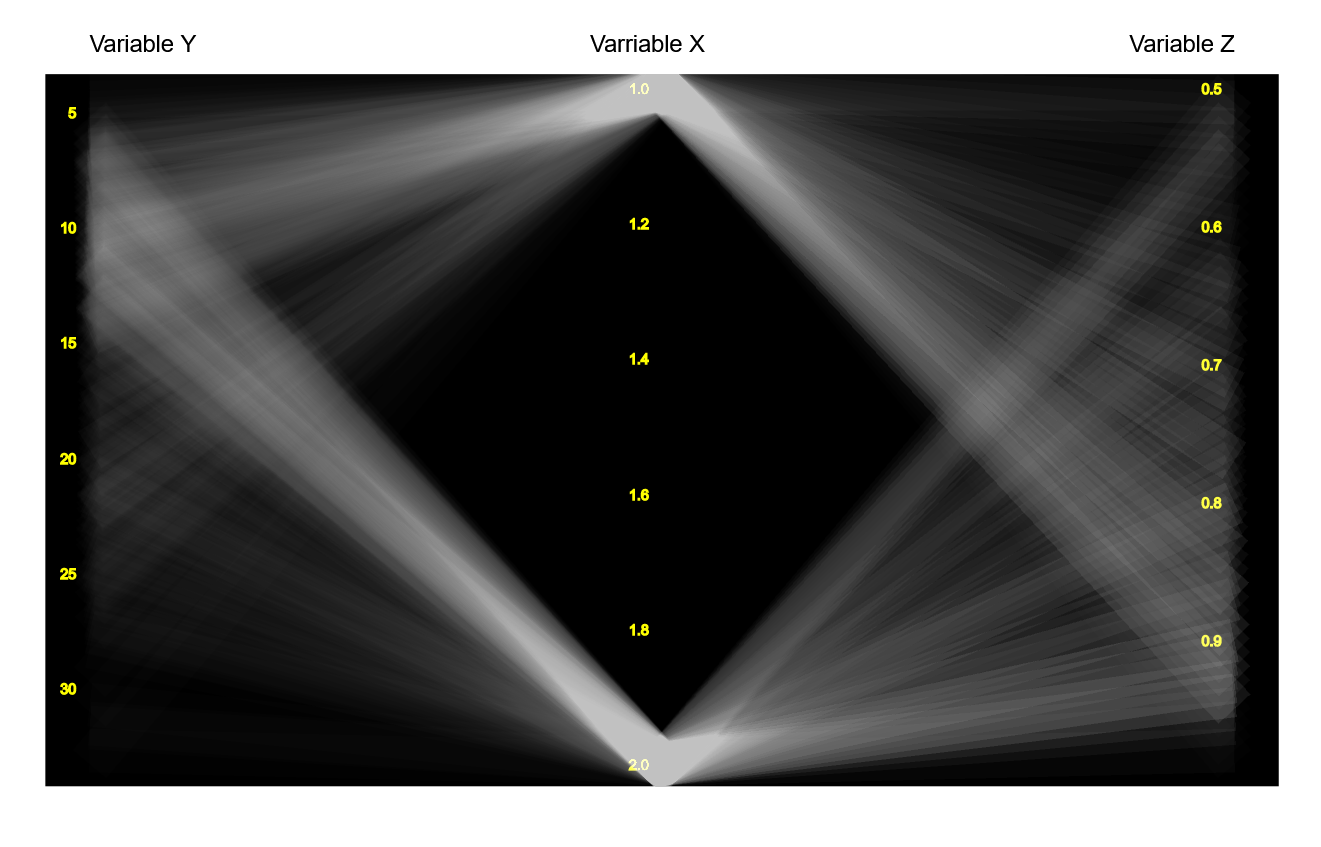
\includegraphics [width = 0.8\textwidth]{ParalleleBSPPixel.JPG}
  \caption{Visualisierung Zwei: Parallele Koordinaten:Pixel 30, RGBA (255, 255, 255, 0.006) }
\end{figure}
Wahrnehmungsprinzipien und Theorie über Informationsvisualisierung verweisen:
Clusterin, Farbwahrnehmung  und Abstrahierung
Alternativ hätte eine Radviz Visualisierung angewandt werden können, diese hätte allerdings den Fokus weg vom zu untersuchendem Hauptattribut gelenkt. Daher ist Sie keine alternative gewesen obwohl Sie die gleichen Daten darstellt und zu ähnlichen Mentalen modellen führt basiert.
Die Visualisierung ist weniger effektiv, da der Anwender verschiedene Kombinationen von Attributen und Pixel ausprobieren muss um sich ein Bild zu machen. Dies ist allerdings auch der Stärke der Visualisierung, da der Anwender sich die Visualisierung so anpassen kann, dass Sie seinen Bedürfnissen entspricht. Hinsichtlich der Expressivität, kann es dazu kommen, dass der Anwender durch Farbgebungen z.b. Rote Linien. Eine nicht intendierte Interpretation erzeugt.

\subsubsection{Visualisierung Drei: Weihnachts Stern} 
Die dritte Visualisierung lässt sich wohl den pixelorientierten Techniken zuordnen. Dabei werden die im Abschnitt Daten erwähnten Verhaltensweisen und Attribute wie Alter, Geschlecht, Koffeinkonsum, Alkoholkonsum, Tabakkonsum und Sporteinheiten kreisförmig um das Hauptattribut angeordnet. Basierend auf ihrer Korrelation zu diesem Hauptattribut werden sie sowohl farblich als auch in ihrer Größe modifiziert. Die in Visualisierung 2 hinzugefügten Attribute können ebenfalls integriert werden. Somit wird die Korrelation doppelt dargestellt. Die Farbgebung erfolgt durch die Skalierung der Korrelation auf ein Farbschema: negativ wird durch Rot dargestellt, positiv durch Grün. Die Intensität der Farbe wird positiv durch die Korrelation beeinflusst, während der Betrag der Korrelation die Größe des Kreises beeinflusst. Dadurch werden Daten mit hoher Korrelation besonders hervorgehoben. Um die Expressivität beizubehalten, sind die Merkmale und ihre Korrelation als Schriftzug eingefügt. Es sollte jedoch beachtet werden, dass eine qualitative Interpretation suggeriert werden könnte. In der Abbildung ist beispielsweise die Anzahl der Erwachungen dargestellt.

\begin{figure}[h]
  \centering
  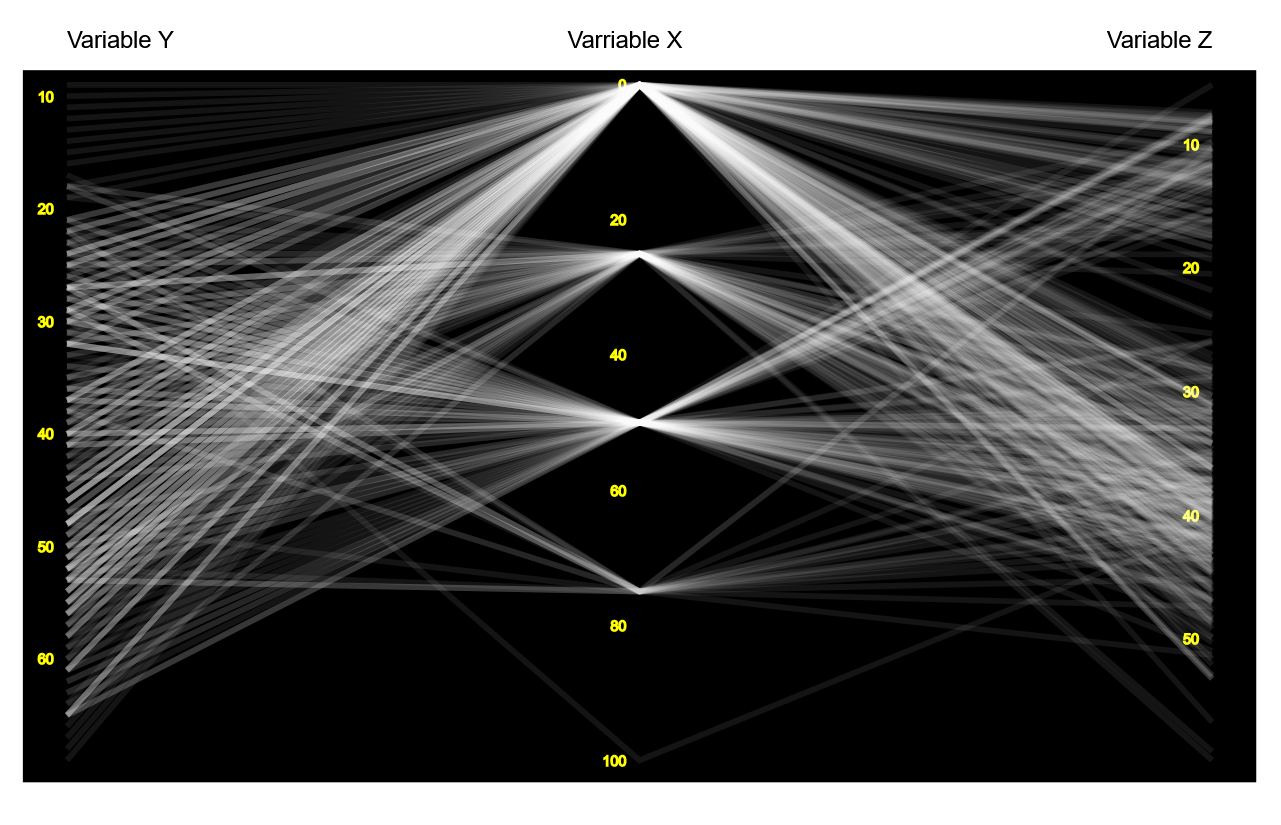
\includegraphics [width = 0.8\textwidth]{RoengtenBSP.JPG}
  \caption{Visualisierung Drei: WeihnachtsStern: Anzahl Erwachungen }
\end{figure}

Obwohl das Erwachen in der Nacht keine Steigerung der lebensqualität ist, könnte angenommen werden, dass die geröteten Attribute grundsätzlich Negativ sind.

Der Anwender kann somit mithilfe dieser Visualisierung schnell Rückschlüsse auf den Einfluss des Verhaltens auf das untersuchte Hauptattribut ziehen. Wichtig dabei ist zu verstehen, dass Korrelation nicht gleichbedeutend mit Kausalität ist.
Alternativ hätte eine Korrelationsmatrix genutzt werden können um die Korrelation darzustellen. Dies wäre auch zu einem änhöichen Mentalem Modell geführt.

\subsection{Interaktion}
Die Visualisierungen sind durch Interaktion miteinander verknüpft. Da es sich um eine Onepage Application handelt ist die 
Interaktion über die Einstellungen umgesetzt um so unötiges klciken zu vermeiden.

In dem Scatterplott kann das Hauptattribut ausgewählt werden und der Datenbereich eingeschränkt werden. 
Diese setzt also den Fokus für die weiteren Visualisierungen.

Die Einschränkung wird auf die verwendeten Daten in den anderen Visualisierungen angewendet so dass nur relevante Daten dargestellt werden.

Das in 1. gewählte attribut wird  Hauptattribut in dem ParalleleM koordinatem System auf die X position angeordnet.
In Visualisierung 2 können zwei weitere  Attribute hinzugefügt werden. Diese werden in Vis 1. als Junior QQ Plotts dargesetellt.

Die dritte Visualisierung wird durch die beiden anderen beeinflusst. So ist das in Vis 1 gewählte Attribut das Hauptattribut auf das korreliert wird und die in Vis 2 gewählten Attribute werden als zusätzliche Zapfen dargestellt.


\section{Implementierung}


Die Visualisierung ist als One-Page-Application konzipiert, was aufgrund der benötigten Interaktion mit den Filtern und der häufigen Auswahl der Attribute nützlich ist. Das `Main.elm` ruft zu Beginn die `Init`-Funktion auf, die den Type Alias `Modell` zunächst auf den Standardwert setzt und die Daten einliest. Die Kommunikation mit dem View erfolgt über den Typ `Msg`, der verschiedene Ausprägungen über Änderungen am Modell an die `Update`-Funktion weitergibt. Die `Update`-Funktion gibt die angehängte Information an das Modell zurück. Besonderer Erklärung bedarf hier die Abspeicherung des Datensatzes, dieser wird im Modell direkt als `List (Aussortierte_Daten)` abgespeichert. Der Typ `Aussortierte_Daten` ist ein Tupel, das die Merkmalsausprägungen abspeichert. Hierbei werden nur die ID, Schlafenszeit und die Aufwachzeit als String abgelegt. Die anderen Attribute sind alle in Floats transformiert. Da die Interaktion vor allem durch Projektion und Selektion umgesetzt ist, erfolgt dies in der Anwendung durch die Filter und die Auswahl der Attribute, die im Modell gespeichert werden.

Die im `Main` wichtigste Funktion ist das `View`. Hier werden verschiedene `div` erzeugt, in denen die Interaktionen und Visualisierungen erstellt sind. Die Auswahl der Attribute erfolgt über ein Dropdown. Dieses übergibt einen String an das `Main` und die Variable bezieht mithilfe eines `case`-Handlings den gewünschten Wert. Der in Visualisierung 1 gewählte Filterbereich wird als `daten` an die anderen Funktionen übergeben. Die so gefilterten Daten werden in einzelne Listen aufgebrochen und die benötigten Attribute wieder zusammengesetzt (Funktionen wie `combined...`). Die Daten werden dann im `div` an die in den anderen Modulen definierten Funktionen zum Zeichnen der Visualisierungen übergeben. Optional werden auch Zustände aus dem Modell mit übergeben.

\subsubsection{QQ Plott}
Der QQ-Plott (scatterplott.elm) definiert zwei wichtige Funktionen die erzeugung von Normalverteilten Daten und das zeichnen des Plotts.

Die Funktion `addNV' funtkioniert wie folgt:
\begin{enumerate}
  \item Die Eingabedaten (\texttt{data}) werden nach den $y$-Werten sortiert.
  \item Es werden verschiedene Berechnungen durchgeführt, um die Normalverteilung zu approximieren und Quantile der Daten zu erhalten.
  \item Eine Transformation (\texttt{transformierer}) wird definiert, um Werte von der Normalverteilung auf die ursprüngliche Verteilung zurückzuübertragen.
  \item Die Funktion \texttt{invNormalCdf} berechnet die inverse Normalverteilungskumulative Funktion.
  \item Quantile werden mit Schätzungen verglichen, um Werte auf der Normalverteilung zu erhalten.
  \item Die Daten werden entsprechend transformiert, um die Normalverteilung darzustellen.
  \item Ein QQ-Plot wird erstellt, indem die transformierten Werte gegen die ursprünglichen Datenpunkte aufgetragen werden.
\end{enumerate}

Die Funktion "drawScatterplot" skaliert die Datenpunkte auf ihre relative XY-Position und zeichnet diese in einem SVG. Eine rote Linie wird zwischen dem 25. und 75. Quantilpunkt gezogen, während die schwarze Linie die Funktion f(x)=xf(x)=x indirekt abbildet. Da diese Funktion aus der Übung bekannt ist, wird sie hier nicht weiter erläutert.

\subsubsection{Parallele Koordinaten}

Die Funktion `blackbox' zeichnet die Parallele Koordinaten Visualisierung.

\begin{enumerate}
\item Die Funktion nimmt eine Liste von mehrdimensionalen Punkten (model), Pixelgröße (pixel), sowie RGB- und Opazitätswerte für die Farbe entgegen.
\item Die Min Max werden berechnet um eine Skalierung zu ermöglichen.
\item Die Daten werden auf Ihre basierend auf der Dimension skaliert und auf die entsprechenden Achsen projiziert.
\item Die Verbindungslinien werden zwischen den Punkten an Ihren relativen Positionen gemalt.
\item Die Farbgebung und Opazität der Linien können durch die Parameter rgb1, rgb2, rgb3 und opacity aus dem Main.Model gesteuert werden.
\end{enumerate}

Die Funktionen zur Berechnung der Quantile, hat ungenutzte Funktionen um die Quantile in in einer anderen Art zu berechnen. Diese wurden im Programm belassen, um diese Funktion dem Anwender später zu ermöglichen.

\subsubsection{Weihnachtsstern}
Die Funktion `graph' zeichnet die Weihnachtsstern Visualisierung.

Hierbei werden die Informationen (Hauptattribut, Verhaltensweisen und ausgewählten Attribute) als DatenTyp ImpactGraph übergeben. Dieser Speichert den Namen des Attributes und eine Liste (Name, List (Float))ab. 


\begin{figure}[h]
  \centering
  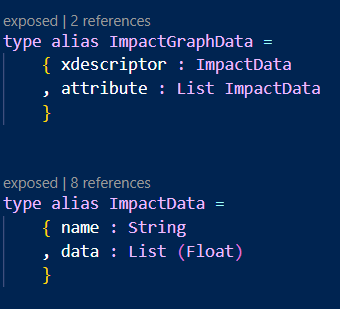
\includegraphics [width = 0.8\textwidth]{ImpactGraphData.JPG}
  \caption{ type Alias ImpactGraphData und ImpactData}
\end{figure}

Hier hervorzuheben ist die reaktive Positionierung der Kreise um das `Hauptattribut' herum.
Die Funktion winkelEinteilung berechnet gleichverteilte Winkelschritte mit : 2 * pi / (length data + 1) 
Die Funtkion Kreis übernimmt diese und weitere relvante Informationen über die Größe und Positionierung der Kreise. 
Hervorzustellen sind hierbei die Funktionen xPosition und yPositon welche basierend auf dem Index einer Liste eine relative Positionierung um den Kreise berechnen. 

\begin{figure}[h]
  \centering
  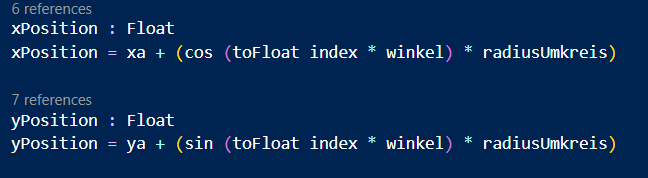
\includegraphics [width = 0.8\textwidth]{Relative XY Positionierung der Kreise.JPG}
  \caption{Relative XY Positionierung der Kreise. }
\end{figure}


Da Elm keine Rückwärts kompatibilität erzwingt, ist es manchmal nicht möglich die neuste version eines Paketes zu verwenden. 
Dies ist allerdings etwas frustrierend, wenn man ein Nützliches paket gefunden hat. Es ist allerdings mögloich den Quellcode auf 
Github, lokal abzuspecihern und als anderes Paket zu importieren, solange die Abhängigkeiten erfüllt sind. Das Modul JXStat ist das Paket Stat aus dem \href{https://github.com/jxxcarlson/elm-stat/blob/6.0.2/src/Stat.elm}{Elm-Stat 6.0.2}. 

Für die Zeichnung des Scatterplott und die Implementierung der Parallelen Koordinaten waren die Übungen sehr hilfreich. Die Implemnetierung der Datenübergabe, Maniulation und auch Visuell anprechende Darstellung war auf persönlicher Ebene am schwierigsten.



\section{Anwendungsfälle}

Im folgendem wird die Anwendung der Visualisierungen anhand von Beispielen erläutert.

\subsection{Anwendung Visualisierung Eins}
 Zu Beginn wird das zu untersuchenende Attribut ausgewählt. In diesem Fall ist es die Schlaf Effizienz. Diese wurde fefiltert auf einen Datenbereich von [0.55; 0.85]
 Hier lässt sich eine gute Annäherung an die Normalverteilung erkennen. Das REM Attribut ist auch annähernd Normalverteilt und hat nur schwache Ausreißer. Der Leichtschlaf Anteils hingegen weist eine schlängerlung auf. Dies ist relevant für die spätere Analyse des Parallelen koordinaten Systems.
\begin{figure}[h]
  \centering
  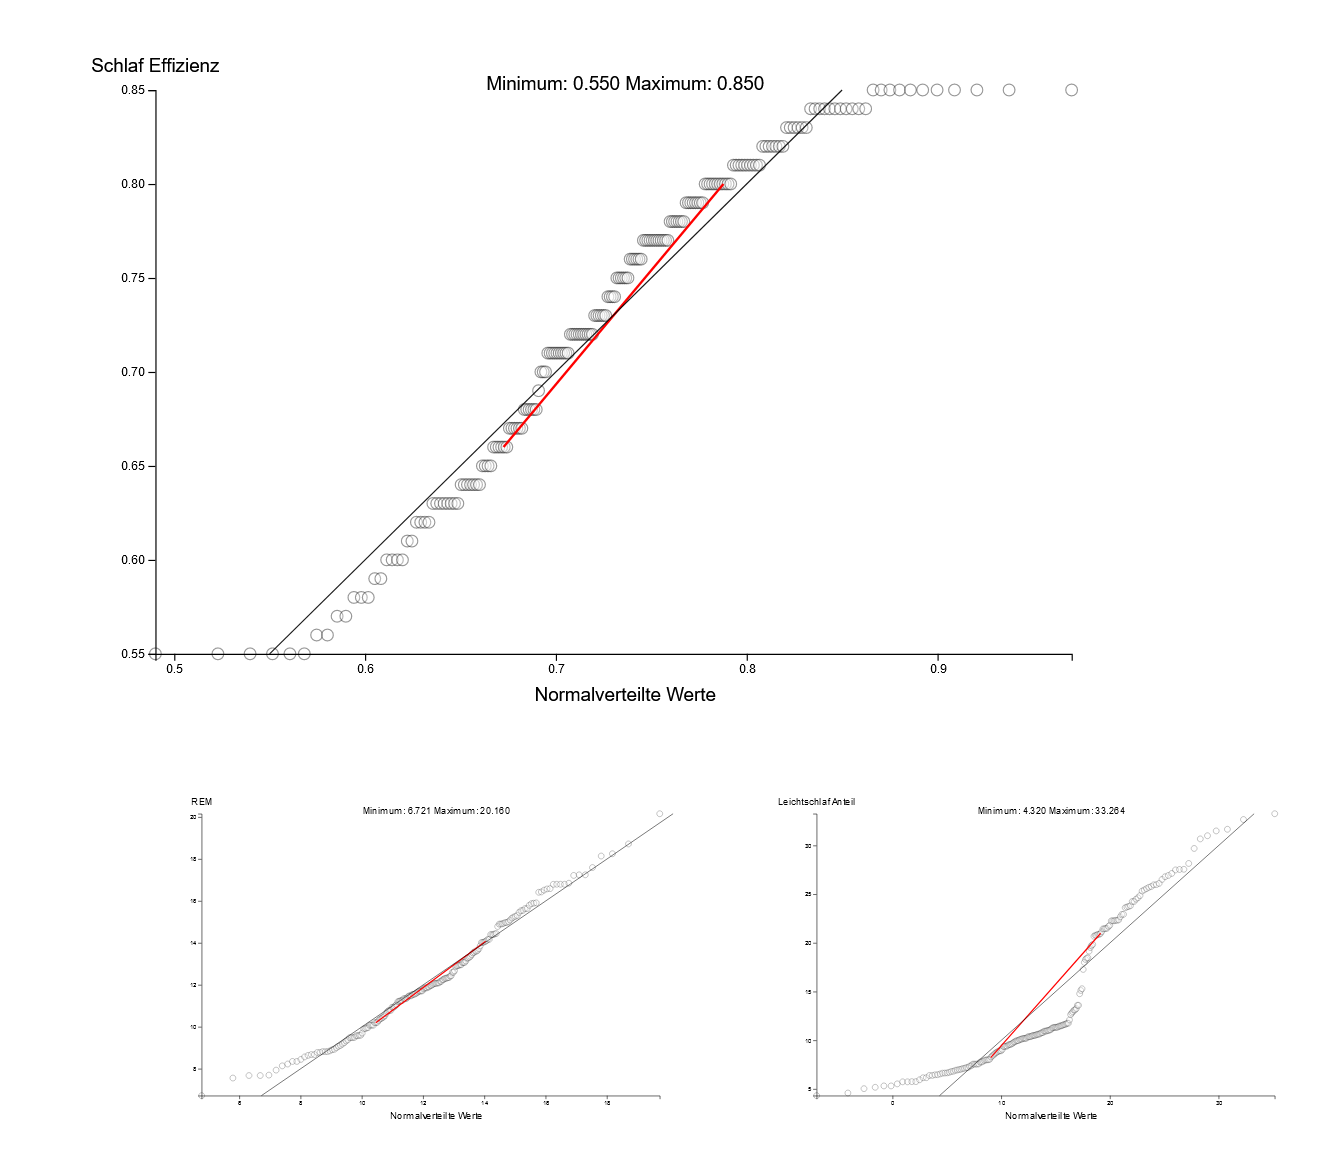
\includegraphics[width = 0.8\textwidth]{Bsp_QQ-Plot.JPG}
  \caption{Visualisierung Eins: Anwendungsbeispiel}
\end{figure}

\subsection{Anwendung Visualisierung Zwei}

Im zweiten Schritt der Visualisierung wurden die Attribute REM und Leichtschalf Anteil untersucht auf Interaktion aufeinander untersucht. Man kann gut erkennen, dass es eine Zusammenhang zwischen niedrigem Leichtenschlaf und hoher Schlafeffizienz gibt. Dies ist allerdings durch die rechts Verschiebung der Daten zu erklären. Bei hohem leichtschlaf Anteil geht ein weiteres Cluster zu einer reduzierten Schlafeffizienz. 
Der Zusammenhang zwische REM und Schlafeffizienz, besteht aus parallel Absenkenden Strichen, dies deutet darauf hin, dass es eine direkte Positive Korrelation zwischen dem REM Schlafanteils die Schlaff Effizienz gibt.

\begin{figure}[h]

  \centering
  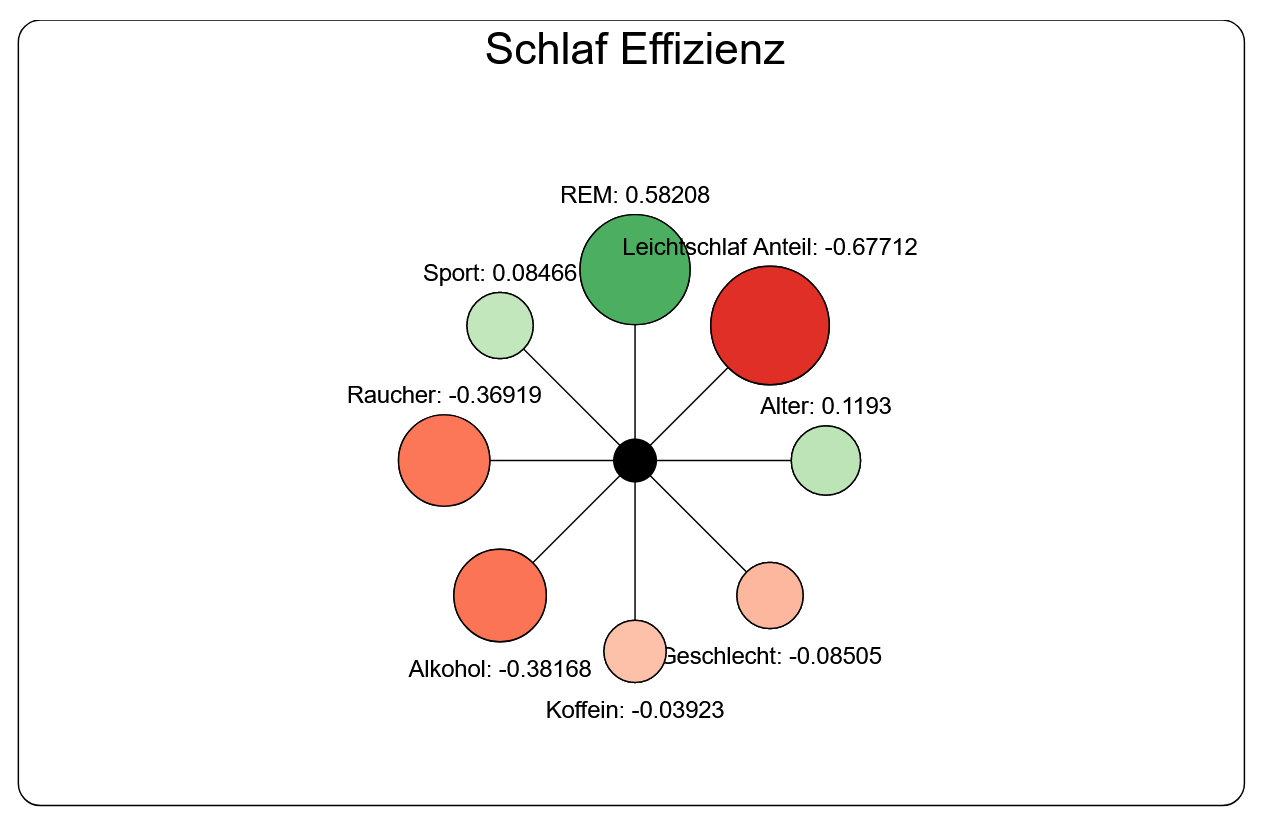
\includegraphics [width = 0.8\textwidth]{Bsp_ImpactGraph.JPG}
  \caption{Visualisierung Eins: Anwendungsbeispiel}

  
\end{figure}

So lässt sich nur aus der Visualisierung ohne Vorwissen die Hypothese entwickeln, dass mit geringerer Schlafeffizienz die REM Schlafanteile sinken und der Anteil des leichten Schlafes erhöht wird.

\subsection{Anwendung Visualisierung Drei}

Die durch Visualisierung 2 entwicklete Hypothese, kann durch Visualisierung 3 unterstützt werden. 
Die Repräsentation der Korrelierung durch die Kugeln  in größe und Farbe zeigen stützen, dass die Korrelation von REM auf die Schlaffeffizienz positiv ist und die korrelation des Leichtschlafanteils negativ. 
Weiter kann man erkennen, dass die Standardmäßig angezeigten Verhaltensweisens Attribute mit der Schlafeffizienz korrelieren. 
Obwohl die Cluster des REM und Leichtschlafes verschieden sind haben Sie dennoch beide einen starken Einfluss auf die Schlaffeffizienz.
Verhaltensweisen wie Alkohol konsum und auch das Rauchen scheinen die Schlafeffizienz zu reduzieren.


\section{Verwandte Arbeiten}
Um eine kurze Literaturrecherche durchzuführen, wurde die Datenbank des ScienceDirect\footnote{\url{sciencedirect.com}} mit dem folgenden Suchstring durchsucht: \newline
{   
    \centering
    \framebox[\textwidth]{
      \label{suchstring}
        \parbox{\textwidth}{
            \centering
            (
                \enquote{informationvisualization} $\lor$ \enquote{visual analytics}
            ) $\land$ (
                \enquote{sleep} $\lor$ \enquote{sleep data} $\lor$ \enquote{sleep efficiency}
            )
        },
    }
}
\newline
Um die gefundenen Ergebnisse weiter einzugrenzen, wurden lediglich Artikel aus dem aktuellen Jahr 2023 betrachtet, 
welche über das für diese Anwendung passende Journal \enquote{Sleep Health} veröffentlich wurden. Im Folgenden werden die beiden Artikel \enquote{Race and sex differences in the longitudinal changes in multidimensional self-reported sleep health characteristics in aging older adults} von Tapia et al.\cite{Tapia2023} und \enquote{The thief of (bed)time: Examination of the daily associations between bedtime procrastination and multidimensional sleep health} von Carlson et al.\cite{Carlson2023} betrachtet.
\newline
Zwei unabhängige Studien zum Thema Schlafgesundheit wurden analysiert, wobei Gemeinsamkeiten und Unterschiede hervorgehoben wurden.
 Die erste Studie von Tapia et al. umfasste eine umfangreiche Stichprobe von über 3000 Teilnehmern und legte besonderen Fokus auf
  demografische Merkmale wie Geschlecht und Rasse. Deskriptive Statistiken wurden präsentiert, wobei Teilnehmermerkmale wie Bildungsniveau,
   Alkoholkonsum und der frühe sozioökonomische Status berücksichtigt wurden. Die Studie analysierte Schlafgesundheitsdimensionen wie Schlafzufriedenheit, 
   Tagesmüdigkeit, Probleme beim Ein- und Durchschlafen sowie die Schlafdauer. Interessanterweise wurden signifikante Wechselwirkungen zwischen Alter, Geschlecht und Rasse identifiziert, die Auswirkungen auf verschiedene Schlafcharakteristika hatten.
\newline
Die zweite Studie von Carlson et al. konzentrierte sich auf eine kleinere Stichprobe und untersuchte spezifisch 
Schlafprokrastination in Verbindung mit Chronotyp und anderen Schlafgesundheitsmaßen.
 Durchschnittliche tägliche Schlafmessungen wurden präsentiert, und 
 bivariate Korrelationsanalysen zeigten Assoziationen zwischen Schlafprokrastination, Chronotyp und verschiedenen Schlafindikatoren. 
 Multilevel-Analysen verdeutlichten, dass höhere Schlafprokrastinationswerte mit schlechterer Schlafgesundheit auf täglicher 
 Ebene verbunden waren. Interessanterweise unterschieden sich die beiden Studien auch hinsichtlich ihrer Fokussierung auf 
 zusätzliche Variablen; die erste Studie berücksichtigte sozioökonomische und demografische Aspekte, während die zweite Studie tiefer
  in die Untersuchung von Schlafprokrastination eintauchte.
\newline
Zusammenfassend reflektieren diese Studien die Vielfalt der Fragestellungen in der Schlafforschung. Während die erste einen breiten Überblick über die Schlafgesundheit unter Berücksichtigung verschiedener Einflussfaktoren bot, konzentrierte sich die zweite auf die detaillierte Analyse von Schlafprokrastination und deren Beziehung zu anderen Schlafcharakteristika. Beide trugen zum Verständnis der komplexen Zusammenhänge bei, betonten jedoch unterschiedliche Schwerpunkte in Bezug auf Stichprobengröße, Variablenauswahl und Analysemethoden.

\section{Zusammenfassung und Ausblick}
Zusammen fassend lässt sich sagen, dass die Visuslierungen dem Anwender einen hohen Nutzen bei der explorativen Analyse der Daten bieten.
Die 
Was wären mögliche sinnvolle Erweiterungen, entweder auf der Ebene der Visualisierungen und/oder auf der Datenebene?

\section*{Anhang: Git-Historie}

\printbibliography

\end{document}

